\documentclass[tikz,border=3pt]{standalone}
\usetikzlibrary{arrows.meta}
\begin{document}
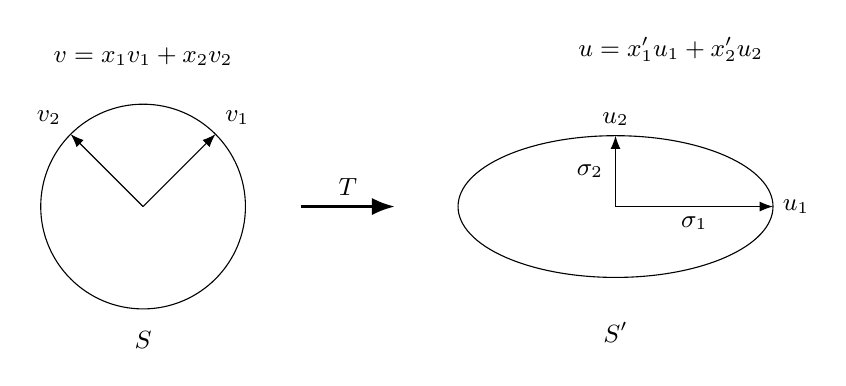
\begin{tikzpicture}[>=Latex, font=\small]
  % --- panel izquierdo: S, base v1,v2 ---
  \begin{scope}
    \draw (0,0) circle (1.3);
    \draw[->] (0,0) -- (0.92,0.92) node[above right] {$v_1$};
    \draw[->] (0,0) -- (-0.92,0.92) node[above left] {$v_2$};
    \node at (0,-1.7) {$S$};
    \node at (0,1.9) {$v=x_1v_1+x_2v_2$};
  \end{scope}

  % --- flecha T ---
  \draw[->, very thick] (2.0,0) -- (3.2,0) node[midway, above] {$T$};

  % --- panel derecho: S', elipse con semiejes sigma1 (u1) y sigma2 (u2) ---
  \begin{scope}[shift={(6.0,0)}]
    \draw (0,0) ellipse (2.0 and 0.9);
    \draw[->] (0,0) -- (2.0,0) node[midway, below] {$\sigma_1$} node[right] {$u_1$};
    \draw[->] (0,0) -- (0,0.9) node[midway, left=1pt] {$\sigma_2$} node[above] {$u_2$};
    \node at (0,-1.6) {$S'$};
  \end{scope}
  \node at (6.7,2.0) {$u=x_1'u_1+x_2'u_2$};
\end{tikzpicture}
\end{document}
